% !TEX root =  main.tex
\fillhack
The high-level goal of \mEdhoc{} is to establish an authenticated security
context for the \mOscore{} security protocol. The overall structure for reaching this goal is a three-message protocol in the style of the \mNoise{} framework, outlined in Figure~\ref{fig:edhocFramework}. In the first message \mMsgone{}, the initiator provides the responder with an ephemeral DH ``half-key'' \mGx{} and, in the \mMethod{} element, suggests authentication methods to be used. The responder may reject the choice of authentication methods.
%
In the second message \mMsgtwo{}, the responder provides its ephemeral
DH half-key \mGy{} and authenticates itself to the initiator by
providing authentication information \mAuthr{}.
%
Finally, in the third message \mMsgthree{}, the initiator authenticates itself to the responder by providing authentication information \mAuthi{}.
%
The authentication information consists of a MAC for all authentication methods. This MAC is also signed when authentication is based on public key signatures.
%
In addition to the exchange of DH half-keys and authentication data, the messages also include parameters for the \mOscore{} security context, such as encryption algorithm identifiers (\mSuites{}) and \mOscore{} security context identifiers \mCi{} and \mCr{}.
%

Optionally, messages may also include application layer data \mAD{}, which enjoys differing levels of protection depending on which message it is part of.
%
As will be described below, when the authentication information is based on a pre-shared key, the \mCredi{} and \mCredr{} credential identifiers are not used. Instead, a single identifier for the pre-shared key is transmitted in message \mMsgone{}.
\begin{figure}[!h]
\centering
\tikzset{>=latex, every msg/.style={draw=thick}, every node/.style={fill=none,text=black}}
\begin{tikzpicture}
    \node (ini) at (0, 0) {Initiator};
    \draw [very thick] (0, -0.5) -- (0,-2.7);
    \draw [very thick] (7, -0.5) -- (7,-2.7);
    \node (res) at (7,0) {Responder};
    \msg{2em}{ini}{res}{\mMsgone: \mMethod, \mSuites, \mGx, \mCi, \mADone};
\msg{4em}{res}{ini}{\mMsgtwo: \mCi, \mGy, \mCr, [\mIdcredr, \mAuthr, \mADtwo]};
    \msg{6em}{ini}{res}{\mMsgthree: \mCr, [\mIdcredi, \mAuthi, \mADthree]};
    \draw [line width=2mm] (-0.75,-2.7) -- (0.75,-2.7);
    \draw [line width=2mm] (7-0.75,-2.7) -- (7+0.75,-2.7);
    \end{tikzpicture}
\caption{Outline of the overall structure of \mEdhoc{}. Elements in square
brackets are encrypted and integrity protected.}
\label{fig:edhocFramework}
\end{figure}

One of the driving design goals is to accommodate three credential types
a party may use to to authenticate itself to peers -- certificates, private keys
and static long-term DH keys. Depending on the credential types used, the authentication methods may differ, and \mAuthi{} and \mAuthr{} need to be constructed accordingly.
%
%As will be clear, it is natural to break down the description of \mEdhoc{} based on the combination of the authentication method used by the initiator and the one used by the responder.
%
The three broad authentication methods are based on digital signatures (\mSig), challenge-response signatures based on static long-term DH keys (\mStat) and pre-shared symmetric keys (\mPsk). The two parties may use different authentication methods in an \mEdhoc{} run.
%
While any combination of the \mSig{} and \mStat{} methods is possible, when \mPsk{} is used, both parties must use \mPsk{}.
%
We refer to these combinations of authentication methods simply as methods to follow the terminology in the \mSpec{}.
%
We denote the methods \mSigSig, \mSigStat, \mStatStat, \mStatSig{} and \mPskPsk.
%
The first authentication method in the name denotes the authentication method used by the initiator of the protocol run and the second denotes the one used by the responder.
%
Parties use mixed types of credentials in \mSigStat{} and \mStatSig{}, so
we often refer to these methods as mixed methods.
%
We refer to a method where at least one party uses \mSig{} as a \mSig-based method and similarly for \mStat{} and \mPsk.
%

To put \mEdhoc{} in context, we first briefly discuss relations to
the protocols on which \mEdhoc{} is based before providing details on the
methods.
%

%-----------------------------------------------------------------------------
\spacehack
\subsection{Relations to \mSigma, \mOptls{} and \mNoise{}}
\label{sec:relationsToOtherProtocols}
\fillhack
\mEdhoc{} uses existing protocols as cryptographic cores to
establish the session key. In this section, we discuss the relationships between \mEdhoc{} and these protocols.
%
%\mEdhoc{} also negotiates parameters (like the encryption algorithm identifiers discussed previously) required for establishing a complete \mOscore{} security context.
%
%Examples of such parameters are encryption algorithm identifiers discussed previously.
%
We note that many key exchange protocols, e.g, \mSigma{}, have an explicit, generic mechanism to securely negotiate such parameters, which other protocols can easily extend. However, they do not always specify exactly how messages and parameters are encoded, which is a requirement for an industrially-standardized protocol like \mEdhoc{}, which needs to negotiate parameters for establishing a complete \mOscore{} security context.
%
%We leave those encoding details out when discussing the relations between \mEdhoc{} and existing protocols.
%

%-----------------------------------------------------------------------------
\spacehack
\subsubsection{\mSigma{}}
\label{sec:sigma}
The \mSigSig{} method of \mEdhoc{} is closely modeled on the \mSigmaI{} variant of \mSigma{}~\cite{sigma}. This variant provides identity protection for the initiator. However, there are some differences, e.g., \mSigSig{} uses Mac-then-Sign like \mTls{} instead of Sign-then-Mac.

Because \mSigSig{} has already been carefully analyzed in~\cite{DBLP:conf/secsr/BruniJPS18}, we will not focus 
on it in this paper. We do however model \mSigSig{} and verify its properties with the same care as for the other methods.
%

%-----------------------------------------------------------------------------
\spacehack
\subsubsection{\mOptls{}}
\label{sec:optls}
The \mStat-based methods use challenge-respsonse signatures using static
long-term DH keys, and proceed along the lines of
\mOptls~\cite{DBLP:conf/eurosp/KrawczykW16}.
%
The challenge-response signature uses an ephemeral DH half-key as a challenge, mixes this half-key with the secret static DH key to generate the session key and a symmetric temporary key to authenticate the session key using an \mAead{}-transform~\cite{DBLP:conf/eurosp/KrawczykW16,aead}.
\vnote{I'm not quite sure what this sentence intends, but it's terribly run-on. Maybe chop it into smaller, less ambiguous ones?}
%
This authenticates one party to the other, which is sufficient for \mOptls, in that it only aims for server authentication.
%
%In \mEdhoc, a party authenticating with with the \mStat{} authentication method essentially acts as an \mOptls{} client and the other party as an \mOptls{} server. 
%
However, unlike \mOptls{}, \mEdhoc{} requires mutual authentication~\cite{ietf-lake-reqs-04}. The \mStatStat{} method can be thought of as interleaving two \mOptls{} sessions, where the second \mEdhoc{} message carries both the response message of the first \mOptls{} session and the request message of the second \mOptls{} session. For the other \mStat{}-based methods, the party authenticating with with the \mStat{} authentication method essentially acts as an \mOptls{} client and the other party (using \mSig{}-based authentication) as an \mOptls{} server. 

 %and achieves this for the \mStat{}-based methods by mirroring the actions, or by using \mSig{}-based authentication for the other party.
%
%
However, there are some differences between \mOptls{} and the \mStat{}-based methods. For instance, \mEdhoc{} reuses the DH half-key as a challenge to save bandwidth, whereas \mOptls{} makes an explicit
point to use distinct elements for the DH half-key and the
challenge, following the principle of separation of concerns.
%

%------------------------------------------------------------------------- sub
\spacehack
\subsubsection{\mNoise{}}
The \mStatStat{} and \mPskPsk{} methods aim to follow the \mNoise{}
framework~\cite{perrin2016noise}.
%
This framework defines how to construct authenticated key exchange protocols,
known as patterns, using static long-term DH keys or pre-shared
keys as credentials.
%
Its goal is to harmonize among the many static long-term key DH 
based key exchange protocols, of which \mOptls{} is one.
%
\mNoise{} specifies how to derive keys, use transcript hashes to ensure
authentication of the message flow among other things.
%

The closest \mNoise{} pattern to the \mStatStat{} method appears to be the
XX pattern.
%

\knote{I don't believe the blue text is true. From the Noise spec it seems to
    me as if the message elements of XX and \mStatStat are exactly the same.
    XX does not describe any encrypted payload. "ee" means "create a DH-key from
    the two DH-half-keys" in \mNoise{}-language.
}
{\color{blue}
It can be seen that the first two messages of \mStatStat{}
correspond perfectly to the first two messages of the XX pattern of
the \mNoise{} framework.
%
However, in the third message, the XX pattern requires
the initiator to send their static key, followed by an encrypted payload using a
key derived from a combination of the static key and an ephemeral key.
%
In \mEdhoc{}, the static key and the payload are both encrypted in the same key, one depending on the key used for the second message, and on the static key of the initiator.
}

\mEdhoc{} does not use all functions of \mNoise{} exactly as prescribed though.
%
For example, \mNoise{} prescribes that the mixHash function, which corresponds
to the transcript hash of \mEdhoc{}, is called on pre-message public keys
during the initialization.
%
This would correspond to that \mEdhoc{} computes a first intermediate transcript
hash doing the same, which is not the case.
%
Another example is that the optional application layer data sent along with
the second message of \mNoise{}

Because of these, and possibly other, discrepancies one cannot automatically
claim claim that \mEdhoc{} enjoys
the same properties as XX -- proofs may depend on functionality that \mEdhoc{}
does not have or performs differently.
%

%------------------------------------------------------------------------- sub
\spacehack
\subsection{Methods of \mEdhoc{}}
\label{sec:methods}
\fillhack
We are now ready to dive into the various methods of \mEdhoc. Although \mCose{} and \mCbor{} are important building blocks of \mEdhoc{}, and we use their terminology in our \mTamarin{} model to better reflect the \mSpec{}, our model does not cover the details of encoding and \mCose{} interfaces.
%
For instance, it suffices for us to consider authenticated encryption with associated data (\mAead{})~\cite{aead} as a function call. Thus, we omit details about \mCose{} and \mCbor{}, and instead refer the reader to~\cite{}. \vnote{We need references here for both COSE and CBOR!}
%

All methods make use of a common key hierarchy, which we describe first. We then describe the methods and how they utilize the key hierarchy.
%

%------------------------------------------------------------------------- sub
\spacehack
\subsubsection{Key hierarchy}
\label{sec:keyHierarchy}

Keys are derived in \mEdhoc{} using \mHkdf{}~\cite{rfc5869}.
%
The interface of \mHkdf{} provides two functions -- \mHkdfExtract{}, which constructs uniformly distributed key material from random input and a seed, and \mHkdfExpand{}, which generates keys from key material and a seed.
%
The seeds are used to bind the key material and keys to certain parameters. Derived keys are then used as input to encryption and integrity protection algorithms.
%
%

The key hierarchy is rooted in the ephemeral DH key \mGxy{}, the combination of the two half-keys \mGx{} and \mGy{}.
%
From this, keys are successively constructed with each transmitted message, weaving in information parties learn as the protocol progresses, culminating in the established session key material.
%
From the session key material, a key exporter based on \mHkdf{} can be used to extract the encryption and integrity keys required for \mOscore{}.
%
Figure~\ref{fig:kdfdiagram} shows an abstract description of the key hierarchy.
%

From \mGxy{}, three intermediate keys \mPRKtwo, \mPRKthree{} and
\mPRKthree{} are derived.
%
Each one of them corresponds to a specific message in the protocol, and from these intermediate keys, encryption and integrity keys for that message are derived.
%
For \mPskPsk{}, the pre-shared key is used as seed for \mPRKtwo. For all other methods the seed for \mPRKtwo{} is empty.
%
In the \mPskPsk{} and \mSigSig{} methods, all three intermediate keys
are the same, i.e., $\mPRKtwo{} = \mPRKthree{} = \mPRKfour$.
%
For the three \mStat-based methods, however, they differ. This is because the intermediate key \mPRKthree{} is dependent on the static long-term key of the party (or parties, if both) using \mStat{}-based authentication.
%

The result of an \mEdhoc{} run is not a key per se, but rather key material from which encryption keys etc can be derived.
\vnote{Diagram from G\"oran had EDHOC-Exporter() in it. We should mention what that does?}

%

%The keys used for the \mAead{} encryptions are augmented with the suffix `e',
%for encrypting the ciphertext, or with the suffix `m', for generating the MAC
%(MACs only feature in the methods involving asymmetric keys). There are four
%keys -- \mKtwom, \mKtwoe, \mKthreem, and \mKthreeae. The suffixes in the names
%of the keys indicate which intermediate keys they are used to generate.
%\mPRKtwo{} is used to generate the key \mKtwoe{} along with the appropriate
%transaction hash. \mPRKthree{} is used for the keys \mKtwom{} and \mKthreeae,
%while \mPRKfour{} is used to generate \mKthreem.

\begin{figure}[!h]
\scalebox{.75}{
% !TEX root =  edhocProtocol.tex
% Start the picture
\begin{tikzpicture}[%
    >=latex,              % Nice arrows; your taste may be different
    start chain=going below,    % General flow is top-to-bottom
    node distance=10mm and 60mm, % Global setup of box spacing
    every join/.style={norm},   % Default linetype for connecting boxes
    ]
% ------------------------------------------------- 
% A few box styles 
% <on chain> *and* <on grid> reduce the need for manual relative
% positioning of nodes
\tikzset{
terminput/.style={rounded corners, text width=6em},
term/.style={rounded corners},
  base/.style={draw, thick, on chain, on grid, align=center, minimum height=6ex},
  prk/.style={base, draw=Red3, fill=Red3!25, rectangle, text width=4em},
  %hkdfext/.style={base, draw=Green3, fill=Green3!25, isosceles triangle, isosceles triangle apex angle=60, anchor=base, shape border rotate=-90, text width=6em},
  hkdfext/.style={base, draw=Green3, fill=Green3!25, rectangle, text width=8em},
  %hkdfexp/.style={base, draw=orange, fill=orange!50, isosceles triangle, isosceles triangle apex angle=60, anchor=base, shape border rotate=-90, text width=6em},
  hkdfexp/.style={base, draw=orange, fill=orange!50, rectangle, text width=8em},
  keyb/.style={base, draw=Blue3, fill=Blue3!25, rectangle, text width=4em},
  % -------------------------------------------------
  norm/.style={->, draw, Blue3},
}
% -------------------------------------------------
% Start by placing the nodes
\node [prk] (p0) {$g^{xy}$};
\node [hkdfext, join] (h1) {\mHkdfExtract};
\node [prk, join] (p2) {\mPRKtwo};
\node [hkdfext, join] (h3) {\mHkdfExtract};
\node [prk, join] (p3) {\mPRKthree};
\node [hkdfext, join] (h5) {\mHkdfExtract};
\node [prk, join] (p4) {\mPRKfour};

\node [hkdfexp, shape border rotate=180, left= 3cm of p4] (h6) {\mHkdfExpand};
\node [keyb, join, left=3cm of h6] (k3) {\mKthreem};

\node [hkdfexp, shape border rotate=180, left= 3cm of p3] (h4) {\mHkdfExpand};
\node [keyb, join, left=3cm of h4] (k2) {\mKtwom};

\node [hkdfexp, shape border rotate=180, left= 3cm of p2] (h2) {\mHkdfExpand};
\node [keyb, join, left=3cm of h2] (k1) {\mKtwoe};

\node [hkdfexp, shape border rotate=180, below= 1cm of h4] (h8) {\mHkdfExpand};
\node [keyb, below=1cm of k2] (k2b) {\mKthreeae};
%\node [draw=none, fill=none, below=0.5cm of h4] (dummy) {};

\draw [->, norm] (p3.south) -- ++(0,-0.58) -- (h8);
\draw [->, norm] (h8) -- (k2b);
\draw [->, norm] (p2) -- (h2); 
\draw [->, norm] (p3) -- (h4); 
\draw [->, norm] (p4) -- (h6);
%\node [term, fill=Green3!25, below = -1.3cm of h1] (h1name) {\mHkdfExtract};
%\node [term, left = 1cm of h1name] (u1) {H1};
%\draw [->, dotted, shorten >=1mm] (u1) -- (h1name);
\node [terminput, right = 1cm of h1] (u1) {Initial salt};
\draw [->, dotted, shorten >=1mm] (u1) -- (h1);

%\node [term, fill=Green3!25, below = -1.3cm of h3] (h3name) {\mHkdfExtract};
%\node [term, left = 1cm of h3name] (u2) {H2};
%\draw [->, dotted, shorten >=1mm] (u2) -- (h3name);
\node [terminput, right = 1cm of h3] (u2) {Additional input};
\draw [->, dotted, shorten >=1mm] (u2) -- (h3);

\node [terminput, right = 1cm of h5] (u3) {Additional input};
\draw [->, dotted, shorten >=1mm] (u3) -- (h5);


%\node [term, fill=orange!50, below = -0.9cm of h2] (h2name) {\mHkdfExpand};
%\node [term, above = 1cm of h2name] (u3) {H3};
%\draw [->, dotted, shorten >=1mm] (u3) -- (h2);
\node [term, above = 1cm of h2] (u4) {\mTHtwo};
\draw [->, dotted, shorten >=1mm] (u4) -- (h2);

%\node [term, fill=orange!50, below = -0.9cm of h4] (h4name) {\mHkdfExpand};
%\node [term, above = 1cm of h4name] (u5) {H5};
%\draw [->, dotted, shorten >=1mm] (u5) -- (h4);
\node [term, above = 1cm of h4] (u5) {\mTHtwo};
\draw [->, dotted, shorten >=1mm] (u5) -- (h4);

\node [term, above = 0.7cm of h6] (u6) {\mTHthree};
\draw [->, dotted, shorten >=1mm] (u6) -- (h6);
\draw [->, dotted, shorten >=1mm] (u6) -- (h8);
%
% ------------------------------------------------- 
% 
%\path (h2.east) to node [near start, yshift=1em] {$n$} (c3); 
%  \draw [o->,lccong] (h2.east) -- (p8);
%\path (p3.east) to node [yshift=-1em] {$k \leq 0$} (c4r); 
%  \draw [o->,lcnorm] (p3.east) -- (p9);
% -------------------------------------------------
% 
%\path (h1.east) to node [near start, yshift=1em] {$n$} (c1); 
%  \draw [o->,lcfree] (h1.east) -- (c1) |- (p4);
%\path (h3.east) -| node [very near start, yshift=1em] {$n$} (c1); 
%  \draw [o->,lcfree] (h3.east) -| (c1);
%\path (p3.west) to node [yshift=-1em] {$k>0$} (c4); 
%  \draw [*->,lcnorm] (p3.west) -- (c4) |- (p3);
%\path (h4.east) -| node [very near start, yshift=1em] {$n$} (c6); 
%  \draw [o->,lcfree] (h4.east) -| (c6); 
%\path (h5.east) to node [near start, yshift=1em] {$n$} (c6); 
%  \draw [o->,lcfree] (h5.east) -| (c7); 
%\path (p4.east) to node [yshift=-1em] {$k \leq 0$} (c7); 
%  \draw [o->,lcfree] (p4.east) -- (c7)  |- (p9);
%\path (p4.west) to node [yshift=-1em] {$k>0$} (c5); 
%  \draw [*->,lcfree] (p4.west) -- (c5) |- (p5);
% -------------------------------------------------
% A last flourish which breaks all the rules
%\draw [->,MediumPurple4, dotted, thick, shorten >=1mm]
%  (p9.south) -- ++(5mm,-3mm)  -- ++(27mm,0) 
%  |- node [black, near end, yshift=0.75em, it]
%    {(When message + resources available)} (p0);
% -------------------------------------------------
\end{tikzpicture}
% =================================================

}
%\caption{Joint key hierarchy for all methods. Diamond shapes denote inputs conditioned on which method $m$ is used. The digits should be interpreted as 0 = \mSigSig, 1 = \mSigStat, 2 = \mStatSig, 3 = \mStatStat. The red boxes below \mGxy{} represent the intermediate key material used for different messages, and the blue left-most boxes represent the keys entering a \mAead{} transform or used for XOR encryption.}
\caption{Joint key hierarchy for all methods. Diamond shapes denote inputs conditioned on the method $m$, with 0 = \mSigSig, 1 = \mSigStat, 2 = \mStatSig, 3 = \mStatStat.}
\label{fig:kdfdiagram}
\end{figure}

With the key hierarchy outlined, we now describe the \mEdhoc{} methods.
%
%As discussed above, the main difference between the methods is how authentication is achieved.
%
%We therefore focus on that.
%
\spacehack
\subsubsection{\mPskPsk{}}
In this method, the initiator and responder are assumed to share a pre-shared key (\mPsk) identified by \mIDPsk.
%
The message sequence is shown in Figure~\ref{fig:edhocpsk}.
%
The first message contains the \mIDPsk{} identifier.
%
The responder obtains the corresponding \mPsk{} and uses that to construct the authentication data (the MAC in the \mAead{} transform) included in the second message.
%
%The authentication data consists of the MAC in the \mAead{} transform used.
%
In the third message, the initiator uses this same technique to authenticate to the responder.
%

The transcript hash \mTH{} tracks the data sent in the messages.
%
One unconventional feature is that the transcript hash lags behind by one message. That is, the second transcript hash \mTHtwo{}, does not cover the content of the second message (similarly for \mTHthree). The reason for this is that \mTHtwo{} cannot cover the output of the \mAead{} transform, since \mTHtwo{} is itself an input to it.
%
This is the same for all methods, but it does not cause any problems with authentication, since the data not covered by the transcript hash is instead MACed or signed.
%

\begin{figure}[!h]
\scalebox{.69}{
\tikzset{>=latex, every msg/.style={draw=thick}, every node/.style={fill=none,text=black}}
\begin{tikzpicture}
    \node (ini) at (0, 0) {Initiator};
    \draw [very thick] (0, -0.5) -- (0,-11);
    \draw [very thick] (11.5, -0.5) -- (11.5,-11);
    \node[below of=ini,fill=white] () {Knows $g,\ \mPsk,\ \mIDPsk,\ \mADone,\ \mADthree$};
    \node (res) at (11.5,0) {Responder};
    \node[below of=res,fill=white] () {Knows $g,\ \mPsk,\ \mIDPsk,\ \mADtwo$};
    \action{4em}{ini}{Generates \mMethod,\ \mSuites,\ \mCi,\ $x$\\$\mGx = g^{x}$};
    \msg{8em}{ini}{res}{\mMsgone: \mMethod, \mSuites, \mGx, \mCi, \mIDPsk, \mADone};
    \action{9em}{res}{$
      \begin{array}{c}
        \text{Generates } \mCr,\ $y$\\
        \mGy = g^{y}\\
        \mTHtwo = \mHash(\mMsgone, g^{y})\\
        \mPRKtwo = \mHkdfExtract(\mPsk, g^{xy}) \\
        \mKtwoae = \mHkdfExpand(\mPRKtwo, \mTHtwo)
      \end{array}$};
    \msg{18em}{res}{ini}{\mMsgtwo: \mCi, \mGy, \mCr, $\overbrace{\mAead(\mKtwoae; \mTHtwo, \mADtwo)}^{\mCipher}$};
    \action{19em}{ini}{$
      \begin{array}{c}
       \mTHtwo = \mHash(\mMsgone, \mGy)\\
       \mPRKtwo = \mHkdfExtract(\mPsk, g^{xy}) \\
        \mKtwoae = \mHkdf(\mPRKtwo, \mTHtwo)\\
        \mTHthree = \mHash(\mTHtwo, \mCipher)\\
        \mPRKthree = \mPRKtwo \\
        \mKthreeae = \mHkdfExpand(\mPRKthree, \mTHthree)
      \end{array}$};
    
    \msg{28em}{ini}{res}{\mMsgthree: \mCr, \mAead(\mKthreeae; \mTHthree; \mADthree)};
    \action{29em}{res}{$
    \begin{array}{c}
    	\mPRKthree = \mPRKtwo \\
        \mKthreeae = \mHkdfExpand(\mPRKthree, \mTHthree)
    \end{array}$};
    \draw [line width=2mm] (-2,-11) -- (2,-11);
    \draw [line width=2mm] (9.5,-11) -- (13.5,-11);
    \end{tikzpicture}}
\caption{The \mPskPsk{} method of \mEdhoc. $\mAead(k; x; y)$ is used to denote
\mAead{} encryption where $k$ is the key, $x$ is associated data to be integrity
protected, and $y$ is the plaintext.}
\label{fig:edhocpsk}
\end{figure}
%------------------------------------------------------------------------- sub
\spacehack
\subsubsection{\mStat-based methods}
\mEdhoc{} provides three \mStat-based methods -- \mSigStat{}, \mStatStat{} and \mStatSig{}. One or both of the initiator and responder authenticate to their peer using their secret static long-term DH key, \mLtki{} or \mLtkr{} respectively.
%

Authentication is achieved using challenge-response signatures that work as follows when the responder authenticates to the initiator.
%
The initiator sends the ephemeral DH half-key \mGx{} as a challenge to the responder in the first message.
%
%To save bandwidth,  sent in the first message also serves as challenge.
%
Upon receiving \mGx{}, the responder exponentiates it by \mLtkr{}.
%
Assuming the discrete logarithm problem is hard in the underlying DH group, only the initiator and responder will be able to compute $\mGx{}^\mLtkr{}$, and this value is woven in to the key hierarchy as depicted in Figures~\ref{fig:kdfdiagram} and \ref{fig:edhocsigstat}.
%
The responder computes authentication data \mAuthr{} in the form of the MAC \mMactwo{} using the \mAead{} transform from \mSuites{} as proposed by the initiator in the first message.
%
The responder then includes \mMactwo{} in the second message.
%
Knowing the secret ephemeral DH half-key corresponding to \mGx{}, and the public static long-term half-key of the responder, the initiator can also compute $\mGx{}^\mLtkr{}$.
%
The initiator assumes that only the responder knows $\mGx{}^\mLtkr{}$, and therefore considers the responder authenticated if the \mAead{} transform completes successfully.
%
When the initiator is authenticating to the responder, the roles are reversed, and \mGy{} takes the place of \mGx{}, \mLtki{} the place of \mLtkr{}, and \mAuthi{} the place of \mAuthr{}. \mAuthi{} is constructed from \mMacthree{}.
%

Independently of whether one party uses \mStat{}-based authentication, the other party may use \mSig{}-based authentication. In that case, the authentication data for that party is constructed using a regular signature.
%

In contrast to the \mPskPsk{} method, in \mStat{}-based methods, each party provides an identifier, \mIdcredi{} and \mIdcredr{} respectively, for the credentials they use.
%
%We now give the specifics for the methods in clarifying message sequence charts.
%

%------------------------------------------------------------------------- sub
\spacehack
\subsubsection{\mSigStat}
The initiator uses the \mSig{} method, authenticating with a signature,
while the responder uses the \mStat{} method, authenticating with a
challenge-response signature.
%
The detailed message sequence chart is shown in Figure~\ref{fig:edhocsigstat}.
%

\begin{figure}[!h]
\centering
%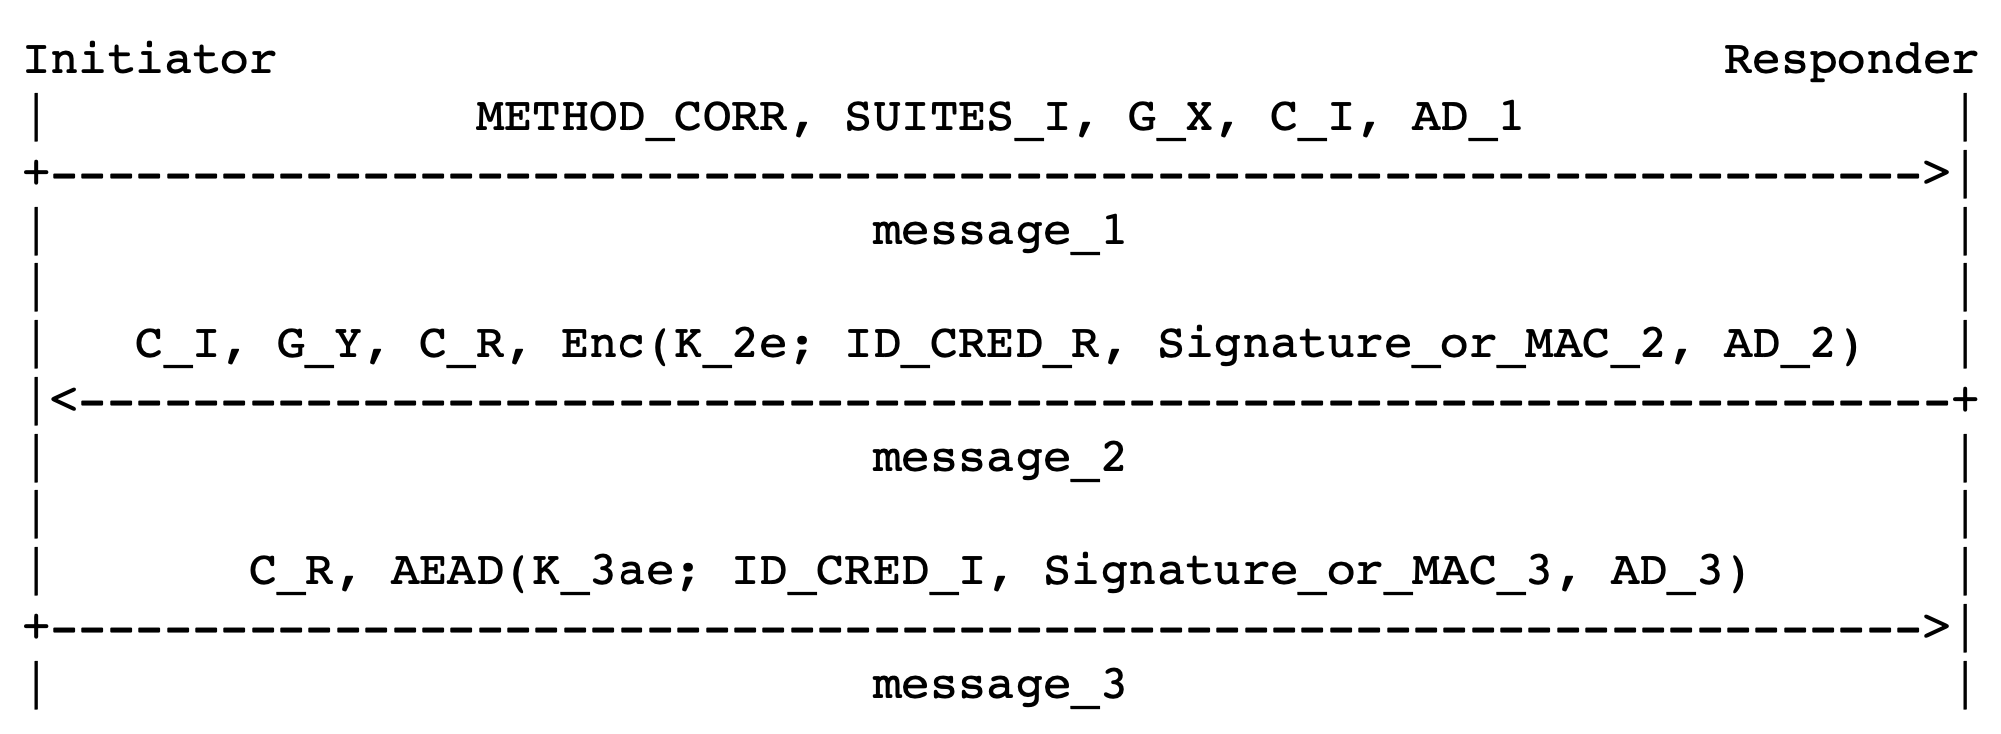
\includegraphics[scale=0.3]{Images/asym.png}
\scalebox{.7}{
\tikzset{>=latex, every msg/.style={draw=thick}, every node/.style={fill=none,text=black}}
\begin{tikzpicture}
    \node (ini) at (0, 0) {Initiator};
    \draw [very thick] (0, -0.5) -- (0,-15);
    \draw [very thick] (9, -0.5) -- (9,-15);
    \node[below of=ini,fill=white] {$
    \begin{array}{c}
    \text{Knows}\ $g$,\ \mCredi,\ \mLtki,\ \mIdcredi,\\
    \mIdcredr, \mADone,\ \mADthree
    \end{array}
    $};
    \node (res) at (9,0) {Responder};
    \node[below of=res,fill=white] {$
    \begin{array}{c}
    \text{Knows}\ $g$,\ \mCredr,\ \mLtkr, \ \mIdcredr,\\
    \mIdcredi, \mADtwo
    \end{array}$};
    \action{5em}{ini}{Generates \mMethod,\ \mSuites,\ \mCi,\ $x$\\$\mGx = g^{x}$};
    \msg{10em}{ini}{res}{\mMsgone: \mMethod, \mSuites, \mGx, \mCi, \mADone};
    \action{11em}{res}{$
      \begin{array}{c}
        \text{Generates } \mCr,\ $y$\\
        \mGy = g^{y}\\
        \mTHtwo = \mHash(\mMsgone, \langle \mCi, \mGy, \mCr \rangle)\\
        \mPRKtwo = \mHkdfExtract(\textrm{``\phantom{}''}, g^{xy}) \\
        \mGrx = \mGx^{\mLtkr} \\
        \mPRKthree = \mHkdfExtract(\mPRKtwo, \mGrx) \\
        \mKtwom = \mHkdfExpand(\mPRKthree, \mTHtwo) \\
        \mMactwo = \mAead(\mKtwom; \langle \mIdcredr, \mTHtwo, \mCredr, \mADtwo \rangle; \textrm{``\phantom{}''}) \\
        \mKtwoe = \mHkdfExpand(\mPRKtwo, \mTHtwo)
      \end{array}$};
    \msg{26em}{res}{ini}{\mMsgtwo: \mCi, \mGy, \mCr, $\overbrace{\mKtwoe\ \mXor\ \langle \mIdcredr, \mMactwo, \mADtwo \rangle}^{\mCipher}$};
    \action{27em}{ini}{$
      \begin{array}{c}
        %\mTHtwo = \mHash(\mMsgone, \langle \mCi, \mGy, \mCr \rangle) \
        \mPRKtwo = \mHkdfExtract(\textrm{``\phantom{}''}, g^{xy}) \\
        %\mKtwoe = \mHkdfExpand(\mPRKtwo,\mTHtwo)\\
        \mGrx = \mCredr^{x} \\
        \mPRKfour = \mPRKthree = \mHkdfExtract(\mPRKtwo, \mGrx) \\
        %\mKtwom = \mHkdfExpand(\mPRKthree, \mTHtwo) \\
        \mKthreeae = \mHkdfExpand(\mPRKthree, \mTHtwo) \\
        \mTHthree = \mHash(\mTHtwo, \mCipher, \mCr)\\
        \mKthreem = \mHkdfExpand(\mPRKfour, \mTHthree) \\
        \mMacthree = \mAead(\mKthreem; \langle \mIdcredi, \mTHthree, \mCredi, \mADthree \rangle; \textrm{``\phantom{}''}) \\
        \mSigthree = \mSign(\mLtki; \langle \mIdcredi, \mTHthree, \mCredi, \mADthree \rangle, \mMacthree \rangle)
      \end{array}$};
    \msg{39em}{ini}{res}{$\mMsgthree: \mCr, \mAead(\mKthreeae; \mTHthree; \langle \mIdcredi, \mSigthree, \mADthree \rangle$)};
    \action{40em}{res}{$
    \begin{array}{c}
        \mTHthree = \mHash(\mTHtwo, \mCipher, \mCr)\\
        \mKthreem = \mHkdfExpand(\mPRKthree, \mTHthree) \\
        \mKthreeae = \mHkdfExpand(\mPRKthree, \mTHthree)
    \end{array}$};
    \draw [line width=2mm] (-2,-15) -- (2,-15);
    \draw [line width=2mm] (7,-15) -- (11,-15);
    \end{tikzpicture}}
    \caption{The \mSigStat{} method of \mEdhoc. \mCredi{} and \mLtki, and
        \mCredr{} and \mLtkr{} are two public-private key pairs. \mCredi{} and
    \mLtki{} must be signature keys in the \mSig{} method. $\mSign(k; x)$ is
    used to denote the signing of message $x$ using key $k$.}
\label{fig:edhocsigstat}
\end{figure}

%------------------------------------------------------------------------- sub
\spacehack
\subsubsection{\mStatStat}
In this method, both the initiator and the responder use the \mStat{}
authentication method.
%
Both parties' secret static long-term DH keys feed into the key hierarchy.
%
The initiator computes authentication data using the \mAead{} transform
and includes that in the third message for the responder to verify.
%
As expected, the initiator's behavior mirrors the \mStat{} authentication method used by the responder in the \mSigStat{} method.
%

%------------------------------------------------------------------------- sub
\spacehack
\subsubsection{\mStatSig}
The \mStatSig{} method is in a sense the mirror of the \mSigStat{} method.
%
Here, the responder runs the \mSig{} method and create the \mAuthr{}
authentication data as a signature over the MAC, while the initiator runs the \mStat{} method.
%
The method is illustrated in Figure~\ref{fig:edhocstatsig}.
%

\begin{figure}[!h]
\centering
%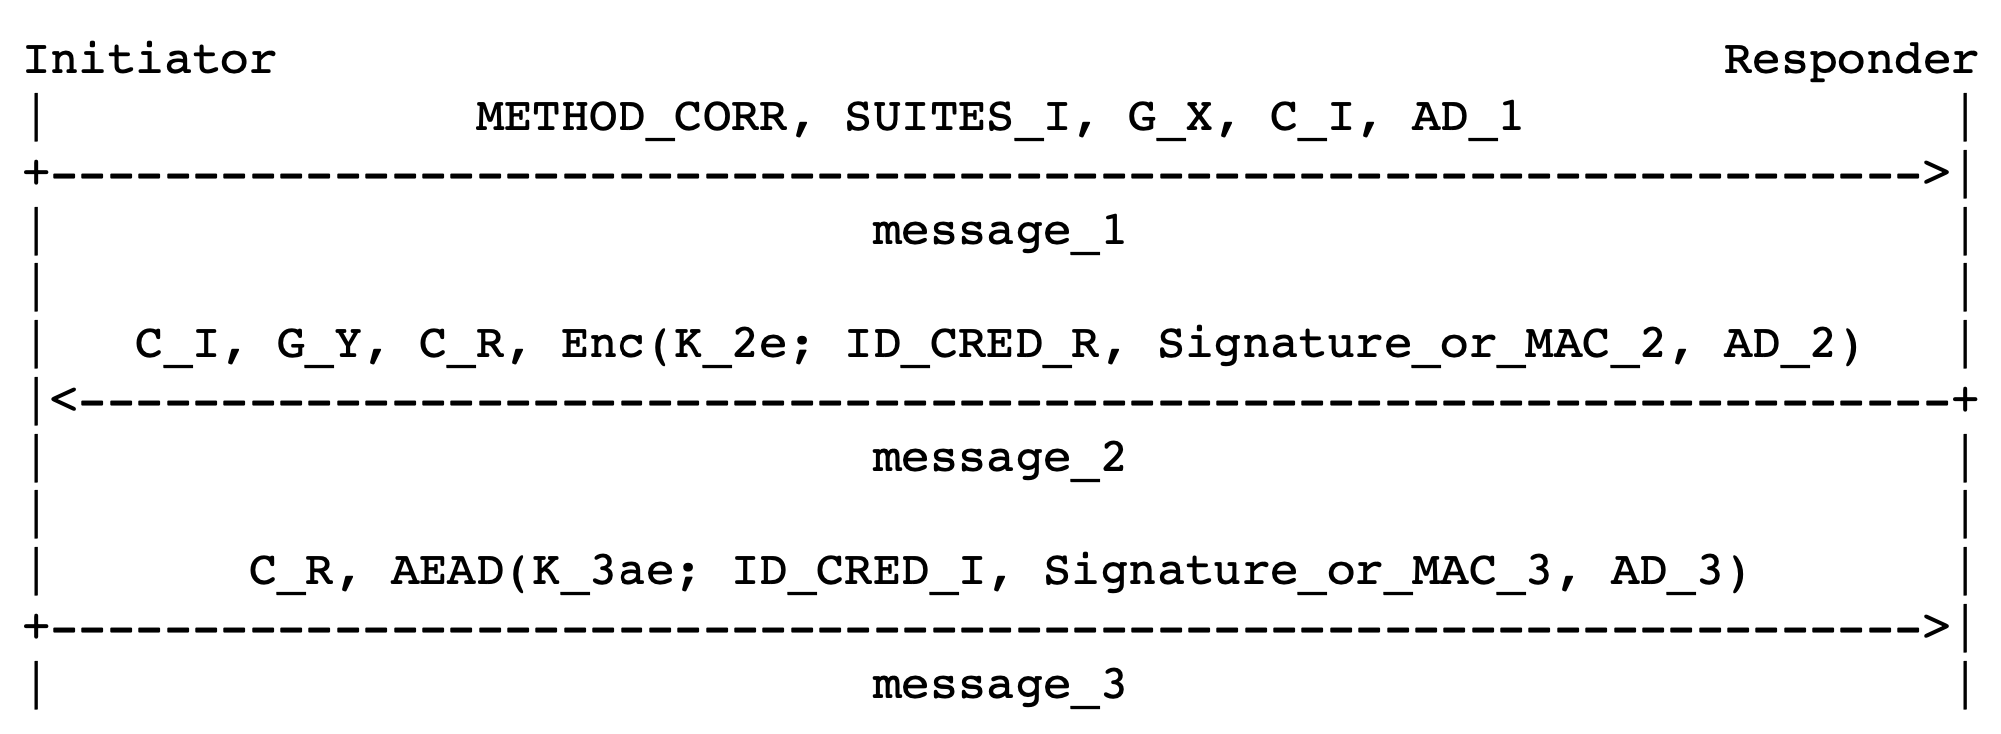
\includegraphics[scale=0.3]{Images/asym.png}
\scalebox{.7}{
\tikzset{>=latex, every msg/.style={draw=thick}, every node/.style={fill=white,text=black}}
\begin{tikzpicture}
    \node (ini) at (0, 0) {Initiator};
    \draw [very thick] (0, -0.5) -- (0,-15.2);
    \draw [very thick] (9, -0.5) -- (9,-15.2);
    \node[below of=ini,fill=white,text=black] {$
    \begin{array}{c}
    \text{Knows}\ $g$,\ \mCredi,\ \mLtki,\ \mIdcredi,\\
    \mIdcredr, \mADone,\ \mADthree
    \end{array}
    $};
    \node (res) at (9,0) {Responder};
    \node[below of=res] {$
    \begin{array}{c}
    \text{Knows}\ $g$,\ \mCredr,\ \mLtkr,\ \mIdcredr,\\
    \mIdcredi, \mADtwo
    \end{array}$};
    \action{5em}{ini}{Generates \mMethod,\ \mSuites,\ \mCi,\ $x$\\$\mGx = g^{x}$};
    \msg{10em}{ini}{res}{\mMsgone: \mMethod, \mSuites, \mGx, \mCi, \mADone};
    \action{11em}{res}{$
      \begin{array}{c}
        \text{Generates } \mCr,\ $y$\\
        \mGy = g^{y}\\
        \mTHtwo = \mHash(\mMsgone, \langle \mCi, \mGy, \mCr \rangle)\\
        \mPRKthree = \mPRKtwo = \mHkdfExtract(\textrm{``\phantom{}''}, g^{xy}) \\
        \mKtwom = \mHkdfExpand(\mPRKthree, \mTHtwo) \\
        \mMactwo = \mAead(\mKtwom; \langle \mIdcredr, \mTHtwo, \mCredr, \mADtwo \rangle; \textrm{``\phantom{}''}) \\
        \mSigtwo = \mSign(\mLtkr; \langle \langle \mIdcredr, \mTHtwo, \mCredr, \mADtwo \rangle, \mMactwo \rangle)\\
        \mKtwoe = \mHkdfExpand(\mPRKtwo, \mTHtwo)
      \end{array}$};
    \msg{25em}{res}{ini}{\mMsgtwo: \mCi, \mGy, \mCr, $\overbrace{\mKtwoe\ \mXor\ \langle \mIdcredr, \mSigtwo, \mADtwo \rangle}^{\mCipher}$};
    \action{26em}{ini}{$
      \begin{array}{c}
        \mPRKthree = \mPRKtwo = \mHkdfExtract(\textrm{``\phantom{}''}, g^{xy}) \\
        \mGiy = \mGy^{\mLtki} \\
        \mPRKfour = \mHkdfExtract(\mPRKthree, \mGiy) \\
        \mTHthree = \mHash(\mTHtwo, \mCipher, \mCr)\\
        \mKthreem = \mHkdfExpand(\mPRKfour, \mTHthree) \\
        \mMacthree = \mAead(\mKthreem; \langle \mIdcredi, \mTHthree, \mCredi, \mADthree \rangle; \textrm{``\phantom{}''}) \\
        \mKthreeae = \mHkdfExpand(\mPRKthree, \mTHthree) \\
      \end{array}$};
    \msg{37em}{ini}{res}{$\mMsgthree: \mCr, \mAead(\mKthreeae; \mTHthree; \langle \mIdcredi, \mMacthree, \mADthree \rangle$)};
    \action{38em}{res}{$
    \begin{array}{c}
       \mGiy = \mCredi^{y} \\
       \mPRKfour = \mHkdfExtract(\mPRKthree, \mGiy) \\
       \mTHthree = \mHash(\mTHtwo, \mCipher, \mCr)\\
        \mKthreem = \mHkdfExpand(\mPRKfour, \mTHthree) \\
        \mKthreeae = \mHkdfExpand(\mPRKthree, \mTHthree)
    \end{array}$};
    \draw [line width=2mm] (-2,-15.2) -- (2,-15.2);
    \draw [line width=2mm] (7,-15.2) -- (11,-15.2);
    \end{tikzpicture}}
\caption{The \mStatSig{} method of \mEdhoc}
\label{fig:edhocstatsig}
\end{figure}

\spacehack
\subsubsection{\mSigSig{}}
In this method, both parties run the \mSig{} method and authenticates with signatures.
%
As mentioned earlier, \mSigSig{} is very closely modeled on \mSigmaI{}, but there are some notable differences.
%
For example, \mEdhoc{} aims to provide some degree of identity protection for responders, and therefore uses the idea from \mSigmaI{} of encrypting the responder identifier \mIdcredr{} (and other items) in the second message.
%
Since bandwidth consumption must be kept down, the designers of \mEdhoc{} consider it wasteful adding a second MAC in addition to the already included \mMactwo{}.
%
\mEdhoc{} applies XOR encryption, with \mHkdf{} being used to generate the key stream.
%
However, \mSigma{} assumes authenticated encryption for this purpose (see Section 5.2 of~\cite{sigma}). 
%


%KARL: we didn't verify anything about this after all. Propose to delete it.

%\subsection{Negotiating a cipher suite and method and correlation parameters}
%\label{sec:ciphersuite}
%Recall that we mentioned that the first message contains a list of cipher suites, ranked according to the preference of the initiator. What does a cipher suite actually contain? An \mEdhoc{} cipher suite consists of an ordered set of \mCose{} algorithms: an \mAead{} algorithm, a hash algorithm, an ECDH curve, a signature algorithm, a signature algorithm curve, an application \mAead{} algorithm, and an application hash algorithm from the \mCose{} Algorithms and Elliptic Curves registries.  
%
%There are four supported cipher suites in \mEdhoc{} -- we refer the reader to Section 3.4 of~\cite{selander-lake-edhoc-01} for the specifics of the algorithms allowed therein. Each cipher suite is identified by one of four predefined integer labels (0--3). Some algorithms are not used in some methods.  The signature algorithm and the signature algorithm curve are not used in methods without signature authentication (i.e. in \mPskPsk{} and \mStatStat).
%
%In order to keep the presentation clean, we have omitted the cipher suite negotiation process from the description of the methods. However, this process happens as follows, at the beginning of every method, once the responder receives the first message. The initiator proposes an ordered list of cipher suites they support. This list presented in descending order to the responder who either accepts the topmost entry in this list (if they also support that suite) or makes a counter-proposal, namely the topmost entry which they support from the remaining part of the list. If there is no such entry the responder can reject, and the protocol does not continue. Similarly, the responder can reject the initiator's choices for the method and correlation parameters as well -- in the case of a reject for either of these values, the protocol aborts.

%------------------------------------------------------------------------- sub
\spacehack
\subsection{Expected security properties}
\label{sec:claimedProperties}
\fillhack
We now identify the security properties that the authors
of the \mSpec{}~\cite{selander-lake-edhoc-01} claim \mEdhoc{} satisfies.
%
We will revisit these claims when we discuss the formal modeling and
verification of \mEdhoc{} in Section~\ref{sec:formalization} and in the
discussions in Section~\ref{sec:discussion}.
\knote{Remember to refer back to this section from formalization section and
    describe which of the properties we model and which we don't (and why?).
    Also refer back to here from the discussion session.
}
%
Many of the claims are imprecisely expressed and some, like KCI, appear to be
described more than once.
%
We elaborate on this in Section~\ref{sec:discussion}.
%
The following list contains our interpretation of the claimed security
properties:
\begin{itemize}
    \item Perfect Forward Secrecy (\textbf{PFS}) for the session key material
    \item Mutual authentication (this presumably refers to entity authentication
        because it is followed by claims of
        \textbf{consistency} (defined in~\cite{sigma}, {\color{red} KARL: I
            believe this definition is equivalent to mutual injective agreement
            on session key, but please double check}
        \textbf{aliveness}, and
        \textbf{peer awareness} to the responder, but not to the initiator)
    \item \textbf{Identity protection} (the initiator against active attacks
        and the responder against passive attacks, except for \mPskPsk{})
    \item Key Compromise Impersonation (\textbf{KCI}) resistance
    \item \textbf{protection against replay attacks} by the attacker (we
    \item A single session of \mEdhoc{} enables the responder to verify
            that the selected cipher suite is the most preferred of the
            initiator which is supported by both parties, even though there is
            no negotiation of cipher suites per se
    \item Compromise of the \mHkdf{} input parameters (\mGxy{} shared
            secret and/or \mPsk) leads to all session keys derived from that
            shared secret being deemed compromised.
            \knote{I don't know which property the above refers to.}
        \item \textbf{Session key independence}
\end{itemize}
%
In this paper, we verify {\color{red} secrecy, authentication, session independence,
perfect forward secrecy, key-compromise impersonation, and some
flavor of post-compromise security.}
%
